\documentclass{article}
\usepackage[utf8]{inputenc}
\usepackage{graphicx}
\usepackage[english,polish]{babel}
\usepackage{polski}
\usepackage{setspace}
\usepackage{url}
\usepackage{hyperref}
\usepackage[numbers]{natbib}
\usepackage{pgf-pie}
\usepackage{pgfplots}

\renewcommand{\baselinestretch}{1.2} 
\setlength{\parindent}{3 em}
\setlength{\parskip}{0.3em}
\pgfplotsset{compat=1.18} 

\begin{document}

\thispagestyle{empty}

\begin{figure}[htbp!]
\centering
%%%          Dla studentów RMS:                                  

\includegraphics[height=5cm]{logoRMS} \\
\end{figure}
\vspace{1.2cm}

\begin{center}
\Large{Dokumentacja projektowa}\\\vspace{0.5cm} \LARGE{\textbf{Inżynieria Biomedyczna w Praktyce}} 

\vspace{2cm}
{\setstretch{1.5}
\large{\textbf{Michał Pawełek}
\\
%% Proszę wpisać nr sekcji projektowej 
%% oraz nazwę specjalności (lub jej skrót) itd.
Sekcja 3, Kierunek: Informatyka \\
Wydział Matematyki Stosowanej \\
Rok akademicki 2021/2022 }\\
\vspace{2.2cm}
\Large{\textbf{Tytuł}: \textit{Ocena poziomu tłuszczu w organizmie na podstawie danych antropometrycznych}}}
\end{center}


\newpage
\setcounter{page}{1}
	\tableofcontents
	\newpage

\section{Wstęp}

W dzisiejszych czasach problemy spowodowane nadwagą przybierają poważniejszego tempa i nie zapowiada się, żeby szybko zniknęły z naszego życia. Najczęściej dotyka to dzieci i nastolatków nie biorący pod uwagę konsekwencji nadmiernego pochłaniania niezdrowego jedzenia. Najczęstszym współczynnikiem nadwagi jest m.in. poziom tłuszczu w organizmie. Oczywiście, jest to bardzo zależna oraz indywidualna skala, na podstawie której nie można wywnioskować precyzyjnych wniosków, lecz dobrze pokazuje w jakim stopniu otyłości może znajdować się pojedyncza jednostka. \\
Celem projektu jest oszacowanie na podstawie wcześniej zmierzonych danych antropometrycznych poziomu tłuszczu w ciele. Granicami wskazującymi czy dana wartość pojedynczej osoby będzie należała do normy, będą dane pochodzące\\z testów analizatora składu ciała znanego pod nazwą InBody. Obiektami przeprowadzonych testów były dzieci oraz nastolatkowie w wieku szkolnym. \\ Po uprzednim uporządkowaniu bazy pod kątem potrzebnych nam danych do właściwej analizy, owe dane będą przekazywane do odpowiednich algorytmów uczenia maszynowego w celu ustalenia własnego poziomu tłuszczu i porównania ich z pierwotnymi wynikami. Dzięki temu będzie można sprawdzić, czy za pomocą otrzymanych wyników antropometrycznych jest możliwość zautomatyzować wskazanie poziomu tłuszczu danej osoby.


\section{Analiza zagadnienia}

Globalny wzrost częstości występowania nadwagi i otyłości we wszystkich kategoriach wiekowych, związanych z brakiem aktywności fizycznej i niewłaściwymi nawykami żywieniowymi, motywuje do badań i uzasadnia skuteczną edukację oraz edukację społeczną jak również zdrowotną, mające na celu złagodzenie tych negatywnych tendencji. Częstość występowania otyłości coraz częściej występuje w niższych kategoriach wiekowych. Otyłość to choroba związana ze zwiększonym poziomem rozwoju gospodarczego kraju oraz charakteryzująca się nadmiernym nagromadzeniem tłuszczu w organizmie człowieka, jest czynnikiem ryzyka wielu chorób niezakaźnych w populacjach dorosłych i dzieci. Ponadto otyłość dziecięca ma tendencję do utrzymywania się w okresie dojrzewania, a nawet w wieku dorosłym, z poważnymi konsekwencjami zdrowotnymi.\\
W związku z narastającą nadwagą, otyłość oraz stan niedowagi w dzieciństwie negatywnie wpływają na sprawność motoryczną, która zależy od koordynacji nerwowo-mięśniowej, sprawności i rozwoju mięśni.
Z nadwagą i otyłością wiąże się nadmiar tkanki tłuszczowej, której ilość mierzy się w celu oceny składu ciała. Tkanka tłuszczowa jest największym narządem dokrewnym w organizmie - jego wzrost prowadzi do poważnych zmian metabolicznych, a w konsekwencji do przemian somatycznych w organizmie. Mięśnie szkieletowe są również bardzo ważne, ponieważ stosunek masy mięśniowej do masy tłuszczowej jest często używany do oceny zdrowia metabolicznego.\\
Najskuteczniejszym sposobem leczenia otyłości u dzieci jest profilaktyka pierwotna. Centralną rolę w profilaktyce odgrywa diagnostyka somatyczna. Poprzez diagnozę somatyczną jesteśmy w stanie określić, a następnie, w trakcie rozwoju, porównać ukierunkowanie wzrostu wybranych parametrów somatycznych dziecka na wykresach centylowych. Jedną z podstawowych metod oceny wzrostu jest porównanie zmierzonych danych antropometrycznych dziecka ze średnią populacyjną za pomocą wykresów wzrostu. Karty wzrostu są nieodzowną częścią praktyki pediatrycznej ze względu na łatwość ich użycia w ocenie wzrostu\\i rozwoju. Badania antropometryczne przeprowadzane w regularnych odstępach czasu są ważnymi wskaźnikami stanu zdrowia dzieci i najwłaściwszym sposobem oceny stanu odżywienia i stanu zdrowia populacji pediatrycznej.\\ \\


Projekt został wykonany w środowisku programistycznym \textit{Jupyter Notebook} przy użyciu języka \textit{Python}. Bazy danych (\textsf{'dane\_inbody' oraz 'dane\_antropo'}) zostały zapożyczone z kursu "Inżynieria Biomedyczna w Praktyce" dla kierunku Informatyka, umiejscowione na Platformie Zdalnej Edukacji należącej do Politechniki Śląskiej. W załączniku do dokumentacji projektu będzie znajdywać się kod projektu w dwóch wariantach: w notebooku (dla odczytania w Jupiterze) oraz w czystym Pythonie (dla jakiegokolwiek środowiska programistycznego umożliwiającym odczyt owego języka)

\newpage

 
 \section{Specyfikacja wewnętrzna}
    \subsection{Przystosowanie bazy danych pod temat projektu}
    Pierwszym jak i najważniejszym krokiem rozpoczynającym każdy projekt jest uprzednie zaimportowanie potrzebnych do pracy bibliotek. W tym projekcie\\w skład wchodziły biblioteki takie jak:
    
    \begin{itemize}
        \item \textbf{numpy,
    	\item pandas,
    	\item seaborn,
    	\item math,
    	\item collections,
    	\item sklearn}.
    \end{itemize}
    Ostatnia z wymienionych jest szczególnie ważna, gdyż dostarczyła najwięcej gotowych funkcji w obszarze klasyfikacji m.in.:
    \begin{enumerate}
            \item różne klasyfikatory (KNN, Naiwny Bayes itp.),
            \item macierz błędów,
            \item metryki,
            \item normalizację zbioru.
    \end{enumerate}
    Po zaimportowaniu bibliotek jak również samych baz danych, potrzebne było wyodrębnić z bazy \textsf{'dane\_inbody'} kolumny zawierającą \textit{BodyFatMass} wraz z jego granicami górnymi oraz dolnymi (wygenerowanymi na podstawie innych danych takich jak chociażby wiek) jak i \textit{id} danego pomiaru.
    \newpage
    
    \begin{figure}[ht!]
		\centering
		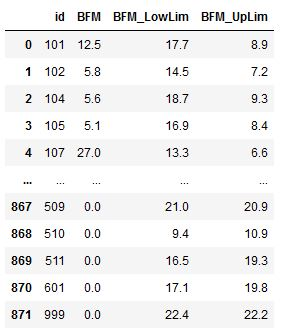
\includegraphics[width=.45\textwidth]{ss/1.JPG}
		\caption{Tablica zawierającą BFM}
		\label{tab:bfm}
	\end{figure}

	Tak stworzona tabela (Rysunek \ref{tab:bfm}) posiada pewne nieprawidłowości - pewne dane nie zgadzają się z nazwą kolumny, dane większe są w kolumnie tam gdzie powinny być mniejsze i na odwrót. Do naprawienia jak również do stworzenia odpowiedniej klasy do klasyfikacji (o czym w następnych krokach) została stworzona autorska klasa (Rysunek \ref{tab:klasa} ).
	
	 \begin{figure}[ht!]
		\centering
		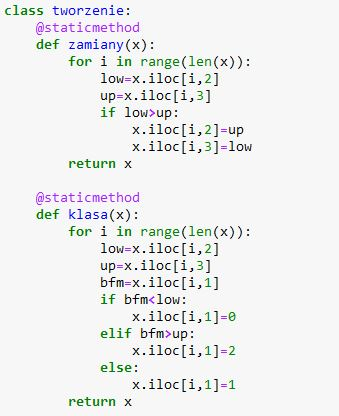
\includegraphics[width=.52\textwidth]{ss/2.JPG}
		\caption{Klasa do zamiany komórek oraz tworzenia klasy}
		\label{tab:klasa}
	\end{figure}
	
	Można łatwo zauważyć, że funkcja \textbf{'zamiania'} to po prostu zmiana kolumny z jednej na drugą w razie złego ustawienia.\\
	Po wykonaniu pierwszej funkcji, w celu ułatwienia oraz ograniczenia się do prawidłowych danych, już od tego momentu należało zacząć redukcję bazy o błędne dane. Z załączonych w \textit{Literaturze} źródeł, zostało określone, że dane o ilości tłuszczu w organizmie dla danej grupy badawczej będą oscylować w granicach nie większych niż 30 oraz nie mniejszych niż 2. \\
	Następnie użyto drugiej z wcześniej wspomnianych funkcji jakim jest \textbf{'klasa'}. Służy ona do ustalenia i nadania odpowiedniej numeracji poziomu tłuszczu. Szacuje ona czy dana wartość mieści się w przedziale poprzednio naprawianym: jeśli wartość jest poniżej dolnego limitu to otrzymuje wartość 0, jeśli jest ona powyżej górnego limitu to 2 a gdy mieści się pomiędzy nimi to dostaje 1. Na podstawie tego sposobu można wstępnie założyć czy dana osoba ma dobry poziom tłuszczu czy odbiega on normy w zależnym od tego kierunku. \\
	Gdy wszystkie rekordy zostały odpowiednio zaklasyfikowane potrzebne było usunąć już niepotrzebne kolumny z granicami jak również przejść do kolejnego kroku jakim było złączenie przygotowanej tabelki wraz z tabelą zawierającą dane antropometryczne. Tabele są łączone poprzez wspólne numery id. \\
	
	\begin{figure}[ht!]
		\centering
		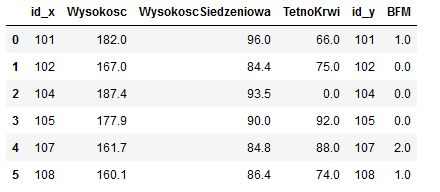
\includegraphics[width=.75\textwidth]{ss/3.JPG}
		\caption{Widok połączonych tabel z wybranymi kolumnami i wierszami}
		\label{tab:baza}
	\end{figure}
	
    Posiadając pełną tabelę z danymi (Rysunek \ref{tab:baza}), należało raz jeszcze zredukować bazę o kolejne niepotrzebne do analizy dane. W tym celu zostały postawione 3 warunki (wszystkie dane zostały dobrane na podstawie źródeł uwzględnionych na samym dole projektu):
    \begin{enumerate}
        \item pomiar miał posiadać ciśnienie skurczowe w granicach od 60 do 181,
        \item pomiar miał posiadać ciśnienie rozkurczowe w granicach 30 do 111,
        \item pomiar miał posiadać tętno krwi od 50 do 110.
    \end{enumerate}
    
    Przy użyciu wcześniej stworzonej zmiennej możemy się dowiedzieć, iż dzięki filtrowaniu usunięto 508 rekordów z 872 a pozostało 364 poprawnych rekordów do analizy, co pokazuje poniższy diagram.\\
    
    \begin{tikzpicture}
        \pie{58.26/ \textbf{Odrzucone próbki},
        41.74/ \textbf{Pozostawione próbki}}
    \end{tikzpicture}\\
    
    Za pomocą funkcji z biblioteki 'Counter', dowiemy się także o ważnej informacji, jaką jest ilość przypisanych pomiarów do odpowiednich klas. Według otrzymanych wniosków (oraz poniższego diagramu), najwięcej pomiarów jest\\w klasie 1, druga w wielkości jest klasa 0 a najmniej znajduje się w klasie 2.\\
    
    \begin{tikzpicture}
        \begin{axis}[
    	xlabel=klasa,
    	ylabel=ilość próbek,
    	enlargelimits=.1,
    	ybar interval=0.8,]
        \addplot 
	    coordinates {(0,133) (1,178) (2,53) (3,20)};
        \end{axis}
    \end{tikzpicture}
    

    \subsection{Normalizacja i podział danych}
    Po usunięciu niepotrzebnych do analizy kolumn takich jak \textit{'id\_x'} czy \textit{'data badania'}, baza danych była prawie gotowa do dalszego działania. Jedyną rzeczą jaką można byłoby jeszcze wykonać przed oddaniem danych pod uczenie maszynowe to  normalizacja zbioru oraz jej podział.\\
    Do tej pierwszej posłużyła funkcja z biblioteki \textbf{'sklearn.preprocessing'} pod nazwą \textit{MinMaxScaler}. Warto ówcześnie pamiętać, że normalizacji nie powinna podlegać sama klasa do klasyfikacji, w tym przypadku to 'BFM'. Aby rozwiązać owy problem wystarczyło zwyczajnie zapisać kolumnę z wcześniej wymienionymi wartościami w pewnej zmiennej, usunąć tę kolumnę z bazy, następnie poddać bazę pod normalizację a na koniec przywrócić zapisaną wcześniej kolumnę z zapisanej zmiennej do już przygotowanej bazy.
    Tak przygotowane dane (Rysunek \ref{tab:norm}) będą poddawane dalszym procedurom.\\
    
    \begin{figure}[ht!]
		\centering
		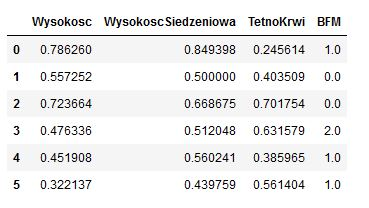
\includegraphics[width=.6\textwidth]{ss/4.JPG}
		\caption{Znormalizowana tabela z wybranymi kolumnami i wierszami}
		\label{tab:norm}
	\end{figure}
     Przed rozpoczęciem klasyfikacji zbiór danych należało podzielić na zbiór treningowy i testowy. Pierwszy z nich, traktowany jako znane dane, służył jako punkt odniesienia dla algorytmów uczenia ich. Drugi zbiór traktowany był jako dane wprowadzane do programu w celu ich sklasyfikowania. Dzięki posiadaniu wiedzy o klasach, jakie przypisane były do tych próbek można było porównać je do wyników klasyfikacji i przeprowadzić analizę skuteczności algorytmów. Proporcje podziału zbioru to 7:3.
     \newpage
 
 \section{Wyniki}
    
    Algorytmami do klasyfikowania danych były kolejno: Naiwny Bayes, regresja logistyczna, KNN, drzewo decyzyjne oraz lasy losowe. Wszystkie algorytmy pochodzą z biblioteki \textit{'sklearn'}.\\
    
    \begin{figure}[ht!]
		\centering
		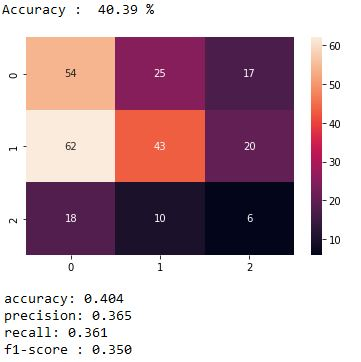
\includegraphics[width=.55\textwidth]{ss/5.JPG}
		\caption{Naiwny Bayes z użyciem wzoru Gaussa}
		\label{tab:nb}
	\end{figure}
	
	\begin{figure}[ht!]
		\centering
		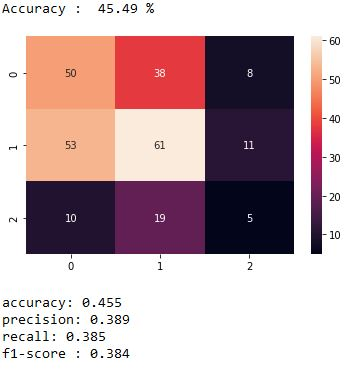
\includegraphics[width=.55\textwidth]{ss/6.JPG}
		\caption{Regresja logistyczna}
		\label{tab:regr}
	\end{figure}
	
	\begin{figure}[ht!]
		\centering
		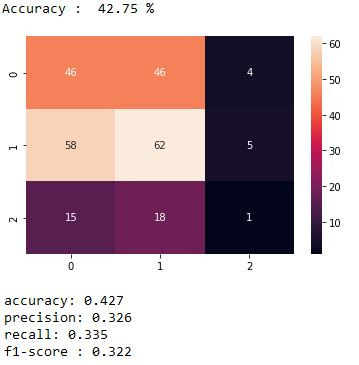
\includegraphics[width=.55\textwidth]{ss/7.JPG}
		\caption{KNN}
		\label{tab:knn}
	\end{figure}
	
	\hspace{5cm}
	
	\begin{figure}[ht!]
		\centering
		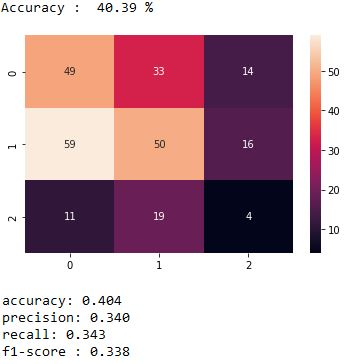
\includegraphics[width=.55\textwidth]{ss/8.JPG}
		\caption{Drzewo decyzyjne}
		\label{tab:tree}
	\end{figure}
	
	\newpage
	
	\begin{figure}[ht!]
		\centering
		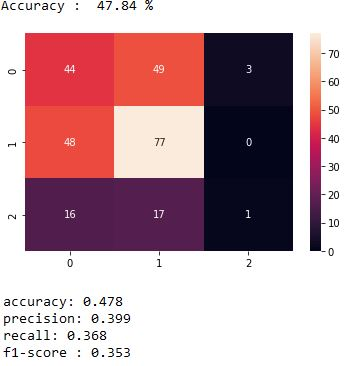
\includegraphics[width=.55\textwidth]{ss/9.JPG}
		\caption{Lasy losowe}
		\label{tab:fore}
	\end{figure}
 
 
    Jak można zauważyć na powyższych macierzach błędów, klasyfikatory miały problem z klasą 2 gdzie ogółem próbek było najmniej. Może to dać do zrozumienia, że dane w tychże próbkach były zbyt bardzo zbliżone np. do klasy 1 i tym sposobem algorytmom mogło obliczać się inny wynik.\\
    Dobrym spostrzeżeniem jest też to, że wszystkie metryki są do siebie bardzo zbliżone - zwłaszcza \textit{'precyzja', 'czułość' i 'f1'}, gdzie wartości oscylują pomiędzy 32\% a 39\%. Świadczy to o specyficzności bazy jak również o braku różnicy skuteczności danej metody.\\
    Żeby uzyskać prawidłowe wyniki, na macierzy musiałyby być liczby tylko na przekątnej zaczynając od lewego górnego rogu, lecz jak widać ani jednemu klasyfikatorowi się to nie udało poprawnie w całości zrobić.
    
    Poniższy diagram (Rysunek \ref{tab:porow}) przedstawia porównanie wszystkich użytych w tym projekcie algorytmów klasyfikacyjnych w formie diagramu słupkowego.
 
 
 
    \begin{figure}[ht!]
		\centering
		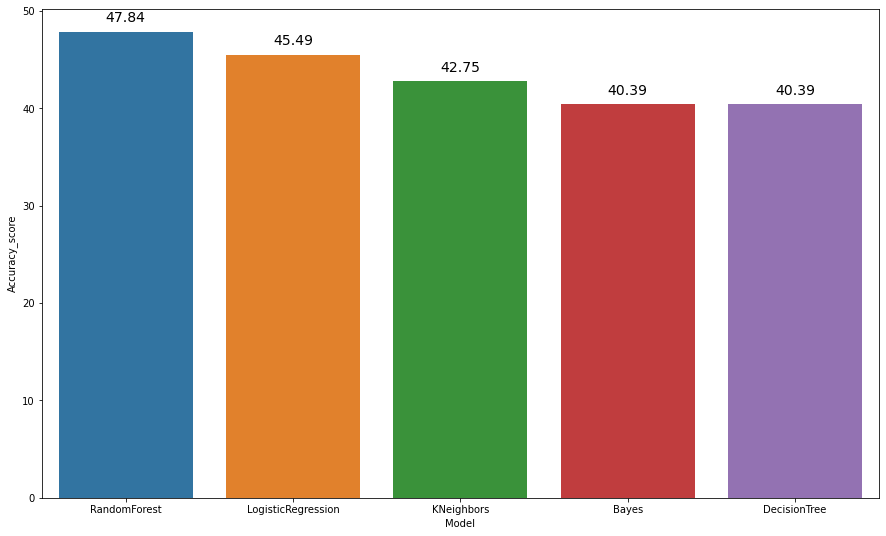
\includegraphics[width=.99\textwidth]{ss/10.PNG}
		\caption{Porównanie klasyfikatorów}
		\label{tab:porow}
	\end{figure}
	
	
 \newpage
 \section{Wnioski}
 
Analizując powyższy diagram mogą się nasunąć dwa wnioski. Pierwszym z nich jest to, że zależność skuteczności pomiędzy danymi algorytmami klasyfikującymi dane na tejże bazie nie jest duża, albowiem nie ma większej różnicy którego algorytmu użyjemy. Może się wydawać przy największym i najmniejszym słupku (\textit{RandomForest i DecisionTree}), iż różnica jest dość znacząca i przekracza około 7\%, ale nie jest to całkowicie prawidłowe spostrzeżenie, gdyż ponownie uruchamiając podział danych wraz z klasyfikatorami będzie można dostrzec znaczącą różnice otrzymanych wyników. Dzieje się tak przez losowy podział zbioru, który za każdym razem inaczej porcjuje dane dla zbioru treningowe jak i testowego.\\
Drugi wniosek dotyczy samej bazy. Posiada ona trudne do uniwersalnego pogrupowania dane. Owe dane są tak mało znacząco zróżnicowane między sobą, że powoduje to trudności podczas klasyfikowania. Nawet po dogłębnym zredukowaniu danych, nie spowodowało to powstaniu idealnej bazy. Jest to oczywiście praktycznie niemożliwe, żeby wszystkie dane (zwłaszcza będące na podstawie prawdziwych badań przeprowadzonych na ludziach) mogły dawać jednoznaczny rezultat.\\
Z obu tych wniosków możemy więc wyciągnąć tezę, która mówi o możliwym, lecz niedokładnym procesie klasyfikowania poziomu tłuszczu przez uczenie maszynowe z danych antropometrycznych.
 
 
 \section{Podsumowanie}
 
 Projekt został zrealizowany całkowicie z ustalonymi wcześniej celami. Głównym celem projektu było oszacowanie poziomu tłuszczu danego uczestnika badania co udało się z powodzeniem. Niestety nie możemy tego powiedzieć o próbie zautomatyzowania procesu przez algorytmy klasyfikujące, ponieważ jak efekt swoich działań był widoczny, tak owe wyniki nie pokrywały się z realnym stanem rzeczy. Dzięki temu można wyciągnąć wnioski, że na tych zbiorach danych nie opłaca się wykonywać uczenia maszynowego. Nie jest to zła wiadomość, lecz blokuje to możliwość dalszego rozwoju w tymże kierunku (ale w innych nadal jak najbardziej pozwala).\\
 Wyniki na poziomie 40\%/50\% nie są zadowalające, zwłaszcza gdy chodzi o klasyfikatory gdzie powinny one być 'górnolotne' - oscylować w okolicach 80\%/100\%. Pomimo tych niedogodności, oficjalnie można oświadczyć że wszystkie cele jakie ten projekt miał dostarczyć zostały spełnione.\\
 Oczywiście dalszy rozwój projektu nie kończy się z oddaniem go do oceny - jest w nim wiele rzeczy, które mogłyby być lepiej zrealizowane oraz bardziej rozszerzone. Jednymi z takich rzeczy są:
 
 \begin{itemize}
     \item Urozmaicenie zakresu danych o inne zbiory np. poprzez przeprowadzenie badań metodą DXA,
     \item Zebranie danych od ludzi z różnych części świata lub różnych sfer społecznych,
     \item Spróbowanie przełożenia projektu na inny język programowania i porównanie wyników,
     \item Lepsze i bardziej precyzyjne redukowanie danych (potrzebne większe doświadczenie w zakresie biologi),
     \item Wykonanie obliczeń klasyfikacyjnych oraz powtórzenie ich np. 100 razy\\i dopiero wtedy spróbowanie wyciągnięcia wniosków.
 \end{itemize}
\newpage


\begin{thebibliography}{9}
        \bibitem{poziom}
            \emph{https://www.builtlean.com/body-fat-percentage-men-women/}
            
        \bibitem{cisnienie1}
            \emph{https://www.mayoclinic.org/diseases-conditions/low-blood-pressure/symptoms-causes/syc-20355465}
            
        \bibitem{cisnienie2}
            \emph{https://apteline.pl/artykuly/prawidlowy-puls-za-niski-puls-tetno-prawidlowe-tetno-spoczynkowe-za-wysoki-puls}
            
         \bibitem{zrodlo1}
            \emph{https://www.mdpi.com/2227-9067/8/5/366/html}
        
        \bibitem{zrodlo2}
            \emph{https://academic.oup.com/advances/article/5/3/320S/4562745}
            
        \bibitem{literatura1}
            Jonathan C. K. Wells
            \emph{Advances in Nutrition,}
             Volume 5, Issue 3, May 2014, Pages 320S–329S
            
        \bibitem{literatura2}
            Bogin.B.
            \emph{Patterns of human growth,}
             Cambridge (UK): Cambridge University Press; 1988

         \bibitem{literatura3}
            Nasreddine, L.; Naja, F.; Chamieh, M.; Adra, N.; Sibai, A.M.; Hwalla, N. Trends in overweight and obesity in Lebanon: Evidence from two national cross-sectional surveys (1997 and 2009).
            \emph{BMC Public Health} 2012.
              
            
    \end{thebibliography}
    \vfill
    Widziane: 10.12.2022

\end{document}
